\documentclass{scrartcl}

% This preamble includes the packages and settings I typically use
% 23.02.22, Robert W

%%% koma script options
\KOMAoption{toc}{bibliography} % insert bibliography in table of contents
\KOMAoptions{
	fontsize=12pt,
	parskip=true,
	%titlepage=false,
	%abstract=false,
	%appendixprefix=true,
}
\addtokomafont{disposition}{\boldmath} % improve math symbols in headings


%%% language settings
\usepackage{polyglossia}
	\setmainlanguage[variant=british]{english}

%%% font
\usepackage{fontspec} 
	\setmainfont{FreeSerif}
	\setsansfont{FreeSans}
	\setmonofont{inconsolata}

%%% hyperref setup
\usepackage{hyperref}
\hypersetup{
	colorlinks=true,
	urlcolor=cyan,
	linkcolor=,
	citecolor=,
	pdfauthor={Robert Wright},
	pdftitle={Preliminary Analysis of Fringilla Insect Data},
}

%%% units (optionally, using version 2)
\usepackage[english,german]{translator} % siunitx needs translator package (not ngerman)! 
\usepackage{siunitx}[=v2]
\sisetup{
	separate-uncertainty=true
}
\NewDocumentCommand{\angsi}{omom}{ % it's now possible to write \angsi{<num>}{\per\second}
	\ang[#1]{#2}\,\si[#3]{#4}
}

%%% bibliography
\usepackage[
	backend=biber,
	style=authoryear-comp,
	bibstyle=authortitle,
	autolang=langname,
	uniquename=init,
	giveninits=true,
	maxnames=2,
	%block=ragged,
	%sorting=none,
]{biblatex}
\AtEveryBibitem{ % don't print url and urldate
	\clearfield{url}
	\clearfield{urlyear}
}


%%% other packages
\usepackage[table,dvipsnames]{xcolor}
\usepackage{csquotes} % quotation marks
\usepackage{mathtools}
\usepackage[onehalfspacing]{setspace}
\usepackage{graphicx}
\usepackage{wrapfig}
\usepackage{float}
\usepackage{pdfpages}
\usepackage{caption}
\usepackage{subcaption}
\usepackage[nameinlink]{cleveref}
\usepackage{booktabs, tabularx, multirow}
\usepackage[roman]{parnotes} % place notes immediately after paragraph
%\usepackage[enable]{easy-todo}
%\usepackage[useregional]{datetime2} % resets date style! FIXME!
%\usepackage[nodayofweek]{datetime} % load after language is set!
	%\newdate{example}{8}{11}{2021}
\usepackage[shortcuts]{extdash} % to hyphenate words with dashes in them
\usepackage[version=4]{mhchem}


%%% costum commands

% Better inline directory listings
\definecolor{light-gray}{gray}{0.95}
\newcommand{\code}[1]{\colorbox{light-gray}{\texttt{#1}}}

% math stuff
\newcommand*\mean[1]{\overline{#1}}
\newcommand{\vect}[1]{\boldsymbol{#1}}


%%%%%%%%%%%%%%%%%%%%%%%%%%%%%%%%%%%%%%%%%%%%%%%%%%%%%%%%%%%%%%%%%%%%%%%%%%%%%%%%%%%
% https://tex.stackexchange.com/questions/16765/biblatex-author-year-square-brackets
\makeatletter

\newrobustcmd*{\parentexttrack}[1]{%
	\begingroup
	\blx@blxinit
	\blx@setsfcodes
	\blx@bibopenparen#1\blx@bibcloseparen
	\endgroup}

\AtEveryCite{%
	\let\parentext=\parentexttrack%
	\let\bibopenparen=\bibopenbracket%
	\let\bibcloseparen=\bibclosebracket}

\makeatother
%%%%%%%%%%%%%%%%%%%%%%%%%%%%%%%%%%%%%%%%%%%%%%%%%%%%%%%%%%%%%%%%%%%%%%%%%%%%%%%%%%%
\addbibresource{/home/robi/research/literature/lit-ibb.bib}
%\listfiles

% TITLE
\titlehead{%
	\centering
\includegraphics[width=0.5\textwidth]{figs/logo-ibb.png} \\
}
\subject{Research Update}
\title{Preliminary Analysis of Fringilla Insect Data}
%\subtitle{}
\author{Robert Wright}
\publishers{Supervisor: Gerard Talavera}
\date{\today}

\begin{document}
	\maketitle
	
	\begin{abstract}
		\noindent
		% HAD TO ADD NEWLINE MANUALLY!
		As part of my internship at the \textit{Botanical Institute of Barcelona}, I have been performing an exploratory analysis on (what I refer to as) the \textit{Fringilla insect dataset}. As far as I am concerned, the data and method of acquisition have been \newline first presented in a paper by \textcite{shapoval2012}. The following report is designed to give an update on the progress of analysis as well as highlight some questions (in \cref{sec:questions}) that came up during the work. All project files can be found on \href{https://github.com/gtlab-barcelona/Robert}{github}.
	\end{abstract}
	\newpage
	\tableofcontents
	
	\section{Data Exploration}

The first step in understanding the insect data is to investigate the yearly abundance. \Cref{fig:total-count} reveals that the data (all traps combined) contains three dominating species: \textit{Vanessa atalanta}, \textit{Inachis io} and \textit{Vanessa cardui}. While \textit{V. atalanta} is recorded consistently in recent years, \textit{V. cardui} and \textit{I. io} show high variation. Most prominently, \textit{I. io} shows pronounced outbreaks in 1985, 2002 and 2011.

\begin{figure}[H]
	\centering
	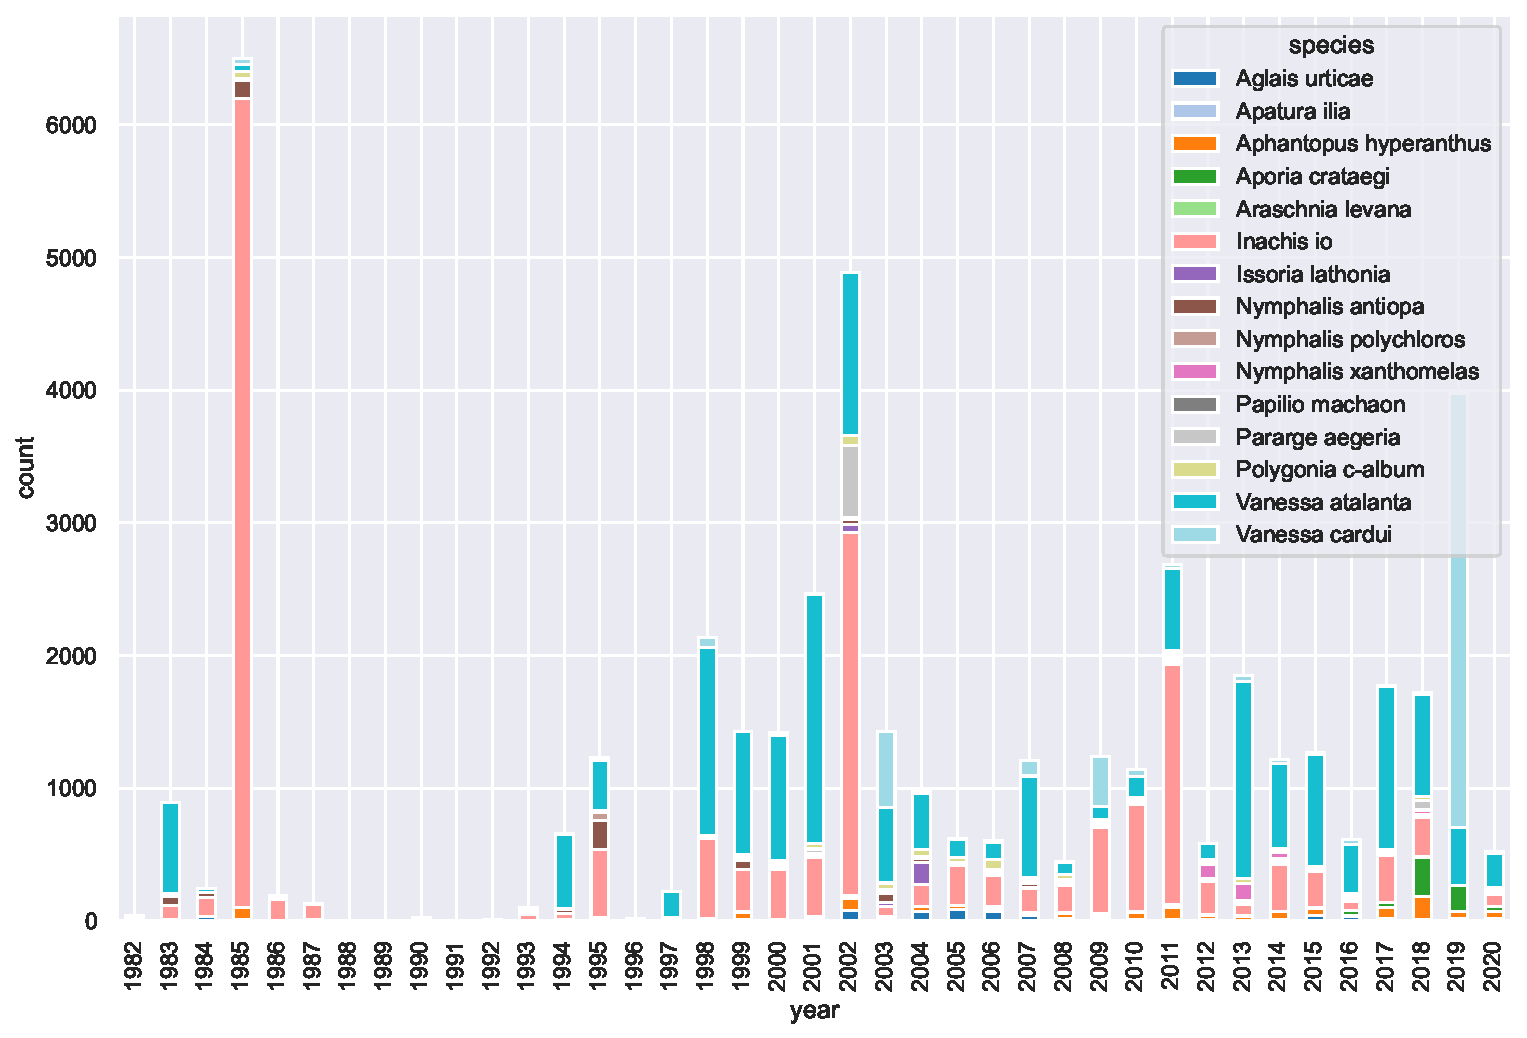
\includegraphics[width=0.9\linewidth]{figs/total-count_per_year_per_species}
	\caption{The total count per year split into single species.}
	\label{fig:total-count}
\end{figure}

\subsection{Missing Values}\label{sec:nans}

The dataset has a high number of missing values in early years, with a considerable \enquote{improvement} from 1998 onwards. Contrary to expectations, the number of missing values in temperature and insect count is not equal. Apparently there have been days in which insect count was monitored, but temperature was not recorded, and vice versa.
Consequently, in order to yield more consistent results, the data analysis is constrained to the time period from 1998 to 2020.

\begin{figure}[H]
	\centering
	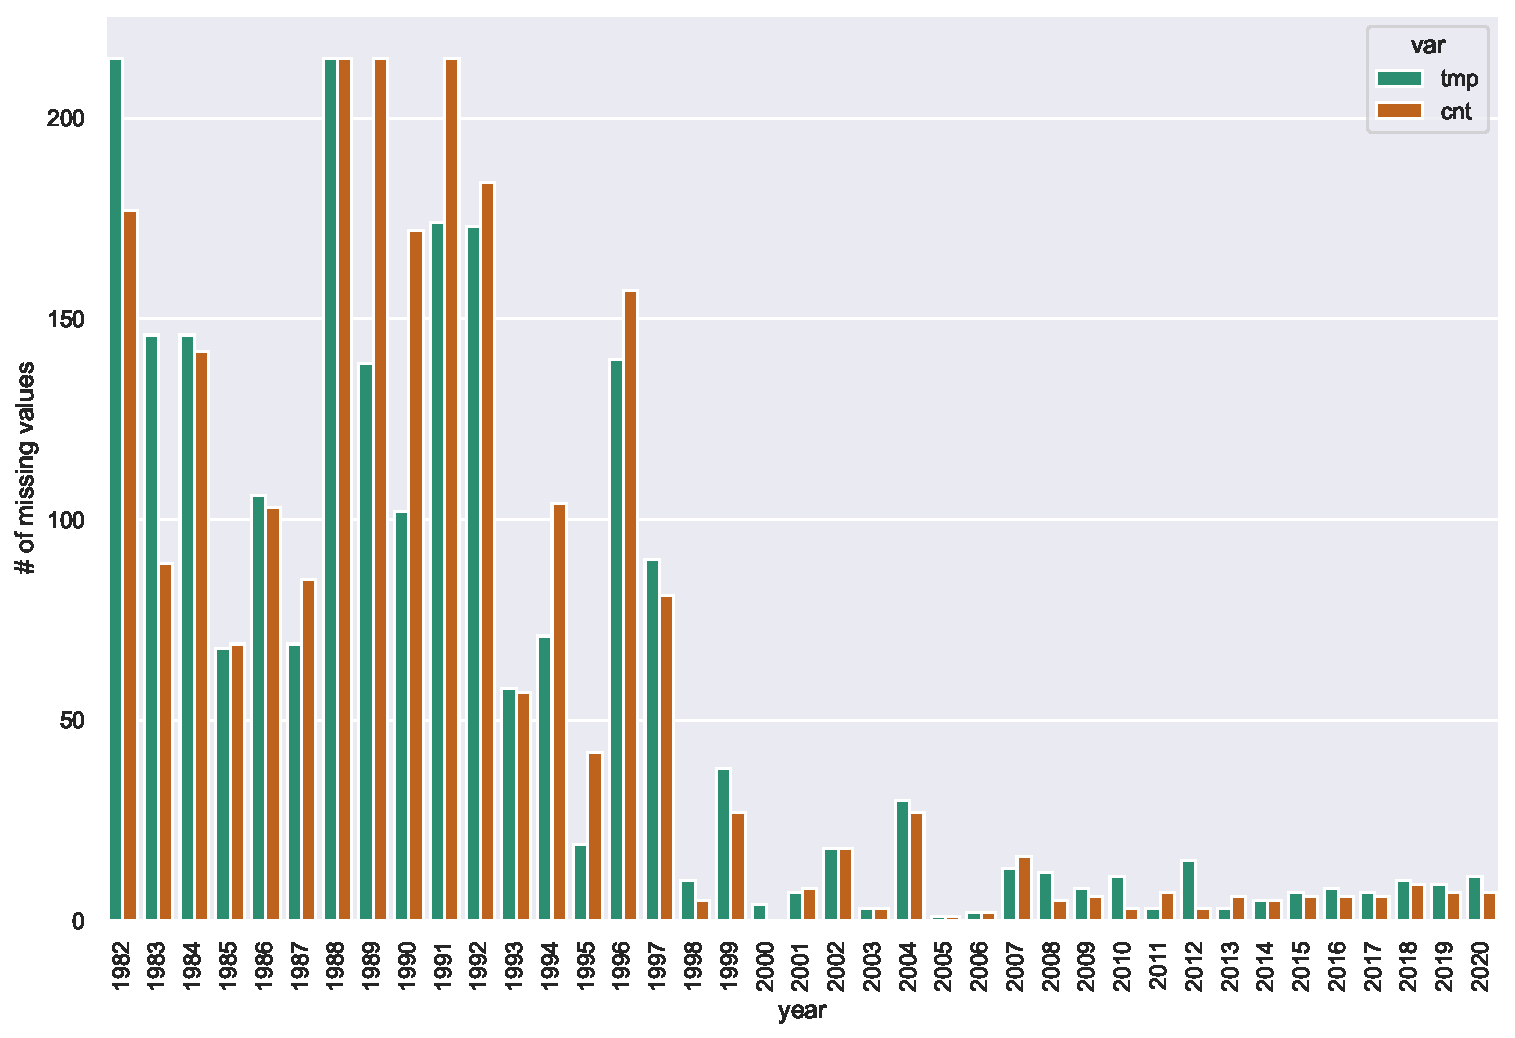
\includegraphics[width=0.9\linewidth]{figs/nans_per-year}
	\caption{Number of missing values in temperature (\textit{tmp}; green) and count (\textit{cnt}, orange) per year.}
	\label{fig:nans-per-year}
\end{figure}
	\section{First Appearance}

Continuing an approach of \textcite{roy2000}, in the following, the timing of first (and last) appearance per year is analysed. Here, the term \enquote{appearance} refers to the earliest (and latest) insect count in the recordings of a single year. In the previously mentioned publication, the authors used data recordings from the \textit{British Butterfly Monitoring Scheme} for the years 1976 to 1998 collected at over 100 sites. Among other things, they found a significant temporal shift to earlier mean first appearances in 13 out of 35 species, including the promising ones from this analysis.

In order to identify linear trends in the Fringilla dataset, a least-squares regression is applied on first appearance with year as the explanatory variable. The fitted model of \textit{I. io} is exemplarily plotted in \cref{fig:io-linregress}, while the results for the remaining species can be found in the attached file as well as \href{https://github.com/gtlab-barcelona/Robert/tree/main/data-exploration_first-last/figs/first-last-day_1998-2020/species}{online}. The statistical parameters of all regressions are summarized in \cref{tab:stats} of \cref{appendix}. It turns out that three species show a significant temporal trend towards earlier appearance: \textit{V. atalanta}, \textit{I. io} and \textit{P. c-album}. However, the data does not reveal a significant relationship for delayed last appearance in recent years for any species.

Proceeding, it would be of interest to relate climate variables to first appearance and investigate the underlying driving factors for the observed change in phenology.
As the Frin- \linebreak gilla data already includes temperature records, starting with the analysis of the influence of temperature on first appearance immediately suggests itself.

\begin{figure}
	\centering
	\includegraphics[width=0.9\linewidth]{"figs/Inachis io_linregress"}
	\caption{\textit{Top:} Total count of \textit{I. io} for the years 1998 to 2020, two outbreaks are visible. \textit{Bottom:} Linear regression on first (orange) and last (green) appearance. Note that the \textit{y}-axis is in days since Jan 1st of the respective year.}
	\label{fig:io-linregress}
\end{figure}

\subsection{Temperature Records}

The Fringilla data includes the daily maximum temperature \parencite{shapoval2012}, however, due to the large number of missing values in early years as well as during the winter months (no monitoring from November to April), comparing the records to and eventually using other sets of temperature data is advisable. A potential replacement dataset might be the \textit{Climate Research Unit gridded Time Series} (CRU TS), covering all land domains (except Antarctica) on a \ang{0.5} latitude by \ang{0.5} longitude grid. This dataset is further discussed by \textcite{harris2020}.
As \cref{fig:annual-mean-tmp} illustrates, the temperature data displays contradictory behaviour: While---speaking of overall trends---the temperature recordings from Fringilla decrease, the annual mean temperature computed from CRU TS becomes warmer. 

\begin{figure}[H]
	\centering
	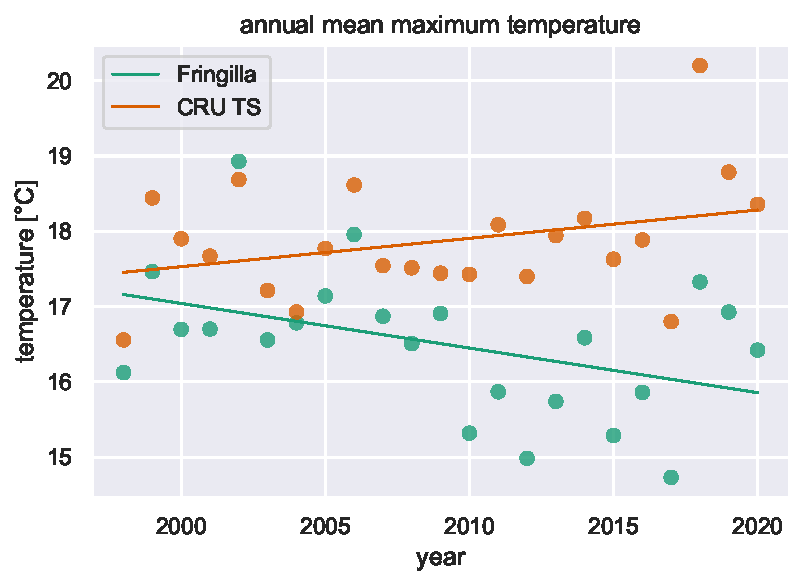
\includegraphics[width=0.9\linewidth]{figs/annual-mean-tmp-comparison}
	\caption{Comparison of the annual mean maximum temperature computed from the Fringilla dataset and CRU TS. Besides the data points, a linear fit is plotted. The annual mean is computed on the closed interval from 1st April to 31st October (\href{https://github.com/gtlab-barcelona/Robert/blob/main/data-exploration_first-last/figs/first-last-day_1998-2020/annual-mean-tmp-comparison.pdf}{image link}).}
	\label{fig:annual-mean-tmp}
\end{figure}


	\section{Open Questions}\label{sec:questions}

To summarize, here is a list of the questions which arose during the exploratory data analysis:

\subsubsection*{Data Exploration}
\begin{itemize}
	\item Does the combination of individual traps introduces any kind of bias to the total count? As \cref{fig:v-atalanta} in \cref{appendix} indicates, some traps were not used throughout the entire period of data acquisition.
	\item The outbreaks of local \textit{I. io} are of interest to us. Were there any attempts you have heard of to find their cause(s)?
	\item The number of missing values decreases drastically after 1997 (see \cref{sec:nans}). Did something fundamentally change in the way the traps were monitored?
\end{itemize}

\subsection*{First Appearance}
\begin{itemize}
	\item According to Fringilla dataset, the temperature is declining in recent years. However, this trend is not supported by CRU TS. Why? Did the method of recording temperature change? 
	Was really the \textbf{maximum} value of daily temperature recorded as stated by \textcite{shapoval2012}?
	\item Is CRU TS an appropriate alternative or do you use any other climate datasets?
	\item What are your thoughts or do you have some general remarks on the analysis of the first appearance? In case you know of any other publication, which might be of interest in this regard, please feel free to share it with us.
\end{itemize}
	\appendix
	\section{Appendix}\label{appendix}

\begin{figure}[H]
	\centering
	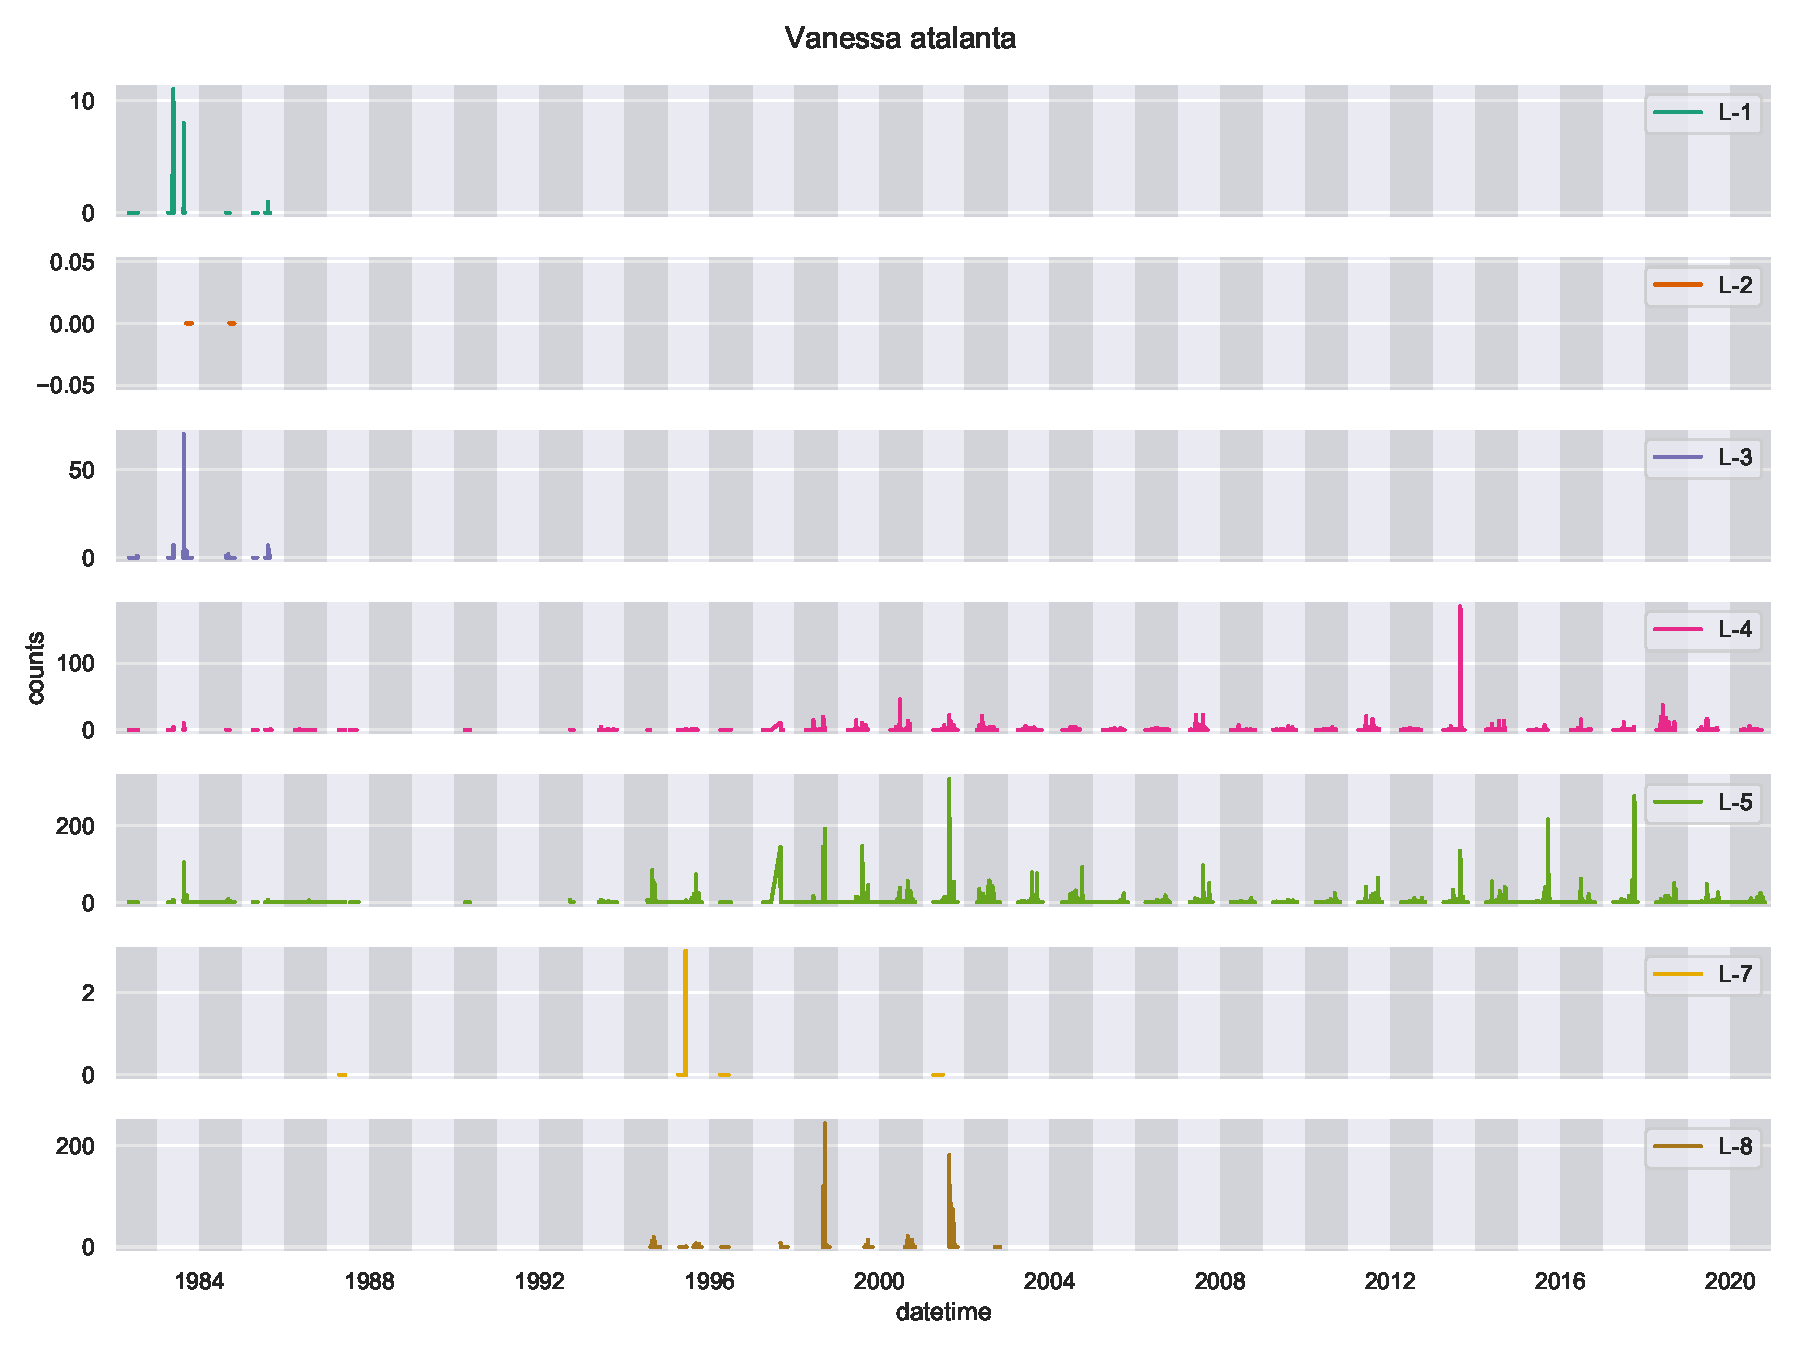
\includegraphics[width=0.9\linewidth]{figs/v-atalanta_single-traps}
	\caption{Daily count of insects caught in individual traps throughout the entire period of time. For illustrative purposes, \textit{V. atalanta} with relatively high abundances was selected, other species can be found \href{https://github.com/gtlab-barcelona/Robert/tree/main/data-exploration_first-last/figs/species_kaliningrad_time-evol_single-traps}{online}. The traps are labelled from \textit{L-1} to \textit{L-8}.}
	\label{fig:v-atalanta}
\end{figure}

%%%

\begin{table}
\centering
\begin{tabular}{@{}ll
		S[table-format=2.1]
		S[table-format=1.3]
		S[table-format=-2.2]
	@{}}
	\toprule
	species & appearance & {\(r^2\) [\%]} & {p-value} & {change (+10y)} \\ \midrule
	Vanessa atalanta & first & 24.0 & \cellcolor{Yellow}0.018 & -13.94 \\
	& last & 1.3 & 0.602 & -1.63 \\
	Vanessa cardui & first & 6.1 & 0.28 & -9.17 \\
	& last & 1.3 & 0.618 & -2.97 \\
	Inachis io & first & 19.7 & \cellcolor{Yellow}0.039 & -4.62 \\
	& last & 0.0 & 0.998 & -0.01 \\
	Issoria lathonia & first & 7.8 & 0.22 & -18.86 \\
	& last & 7.8 & 0.22 & -7.04 \\
	Aglais urticae & first & 12.9 & 0.092 & -28.87 \\
	& last & 0.4 & 0.762 & 1.68 \\
	Aporia crataegi & first & 7.6 & 0.285 & -3.5 \\
	& last & 1.7 & 0.62 & 3.79 \\
	Apatura ilia & first & 9.2 & 0.465 & -5.14 \\
	& last & 94.4 & 0.0 & -41.92 \\
	Aphantopus hyperanthus & first & 3.4 & 0.397 & -2.68 \\
	& last & 4.6 & 0.324 & 2.08 \\
	Araschnia levana & first & 0.2 & 0.884 & 2.66 \\
	& last & 1.4 & 0.686 & 4.49 \\
	Nymphalis antiopa & first & 0.0 & 0.945 & 0.99 \\
	& last & 2.4 & 0.487 & -6.74 \\
	Nymphalis polychloros & first & 12.3 & 0.11 & -15.75 \\
	& last & 1.3 & 0.612 & -6.52 \\
	Nymphalis xanthomelas & first & 14.0 & 0.208 & -32.13 \\
	& last & 0.2 & 0.896 & 3.09 \\
	Papilio machaon & first & 13.0 & 0.276 & -19.57 \\
	& last & 15.6 & 0.23 & 9.84 \\
	Polygonia c-album & first & 20.1 & \cellcolor{Yellow}0.036 & -13.21 \\
	& last & 9.3 & 0.168 & 4.83 \\
	Pararge aegeria & first & 0.4 & 0.81 & 4.11 \\
	& last & 14.1 & 0.138 & -13.05 \\ \bottomrule
\end{tabular}
\caption{Statistical output of regression analysis of linear trend in first and last appearance. The coefficient of determination \(r^2\) is the square of the Pearson correlation \linebreak coefficient. The p-value is derived from a hypothesis test whose null hypothesis is that the slope is zero, using Wald Test with t-distribution of the test statistic. Significance is indicated by yellow filling. Values for change per decade are number of days (\href{https://github.com/gtlab-barcelona/Robert/blob/main/data-exploration_first-last/code/5-stat_output.csv}{csv-file link}).}
\label{tab:stats}
\end{table}


	
	\newpage
	\hypersetup{urlcolor=.}
	%\nocite{*}
	\begingroup
	\setlength{\emergencystretch}{3em}
	\printbibliography
	\endgroup
\end{document}